\newpage
\section{Functional requirements}

The system contains a login function for both caseworkers and applicants. Caseworkers login to the system through an employee portal, while applicants login to the system using NemId. The system validates eligible applicants through NemId.

\vspace{2mm}

Once the applicant is logged in, they are presented with a form through which they submit relevant information. The form contains text input fields and fields through which additional documentation can be attached to the application as pdf files.

\vspace{2mm}

The system assigns submitted applications to available caseworkers at random. Processed applications are archived and saved in an immutable state. Cases are annotated based on their state, i.e. ongoing, archived or on hold. Applications from the same citizen are also annotated in order to detect possible duplicates.

\vspace{2mm}

Once logged in, the caseworker is presented with their assigned cases, as well as a way to search all archived cases. More specifically, the caseworker cannot see ongoing cases not assigned to them, however all archived cases are search-able no matter the assigned caseworker. Caseworkers have access to all data submitted in the cases by the applicant. The caseworker can approve or reject applications. The state of an application is based on a majority vote from the caseworkers, meaning a processed case is assigned to another caseworker until a majority sentiment is met. The system keeps track of individual caseworkers decisions, however does not disclose these decisions to other caseworkers. When the majority vote has been reached, the application is finally either approved or rejected. If the case is approved, the system calculates the "loss of earnings" benefits based on the data contained in the application and the current applicable laws. The system informs the applicant of the final decision, containing the benefits calculations if approved, through an e-mail.

\vspace{2mm}

A caseworker can set an application on hold. In such a case, the applications state must be changed to on hold and the system sends an e-mail to the applicant informing them of the applications state. The caseworker is able to write the message contained in the e-mail. The applicant is able to access the application form through a link in the e-mail.

\vspace{2mm}

A caseworker can be assigned a supervisor role, giving them additional functions. A supervisor is able to see all ongoing and archived cases, as well as which caseworkers has been assigned to which case and the cases current state.
\newpage
\begin{figure}[htb!]
	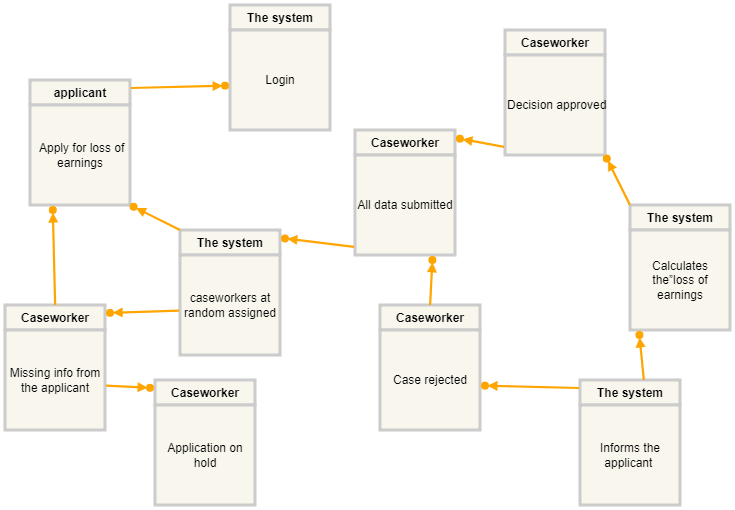
\includegraphics[width=\textwidth]{DCRcopy}
	\caption{DCR graph}
\end{figure}